%
% char2.tex
%
% (c) 2021 Prof Dr Andreas Müller, OST Ostschweizer Fachhochschule
%
\begin{frame}[t]
\setlength{\abovedisplayskip}{5pt}
\setlength{\belowdisplayskip}{5pt}
\frametitle{Charakteristik 2}
\vspace{-15pt}
\begin{columns}[t,onlytextwidth]
\begin{column}{0.48\textwidth}
\begin{block}{Plus und Minus}
\[
x+x = 2x = 0
\uncover<2->{\Rightarrow
-x=x}
\]
\end{block}
\uncover<3->{%
\begin{block}{Quadrieren}
In $\mathbb{F}_2$ ist $2=0$, d.h
\[
(x+y)^2
=
x^2 + 2xy + y^2
\uncover<4->{=
x^2 + y^2}
\]
für alle $x,y\in\Bbbk$
\end{block}}
\uncover<6->{%
\begin{block}{Frobenius-Automorphismus}
\[
(x+y)^{2^n} = x^{2^n}+y^{2^n}
\]
\end{block}}
\end{column}
\begin{column}{0.48\textwidth}
\uncover<5->{%
\begin{block}{Pascal-Dreieck}
\begin{center}
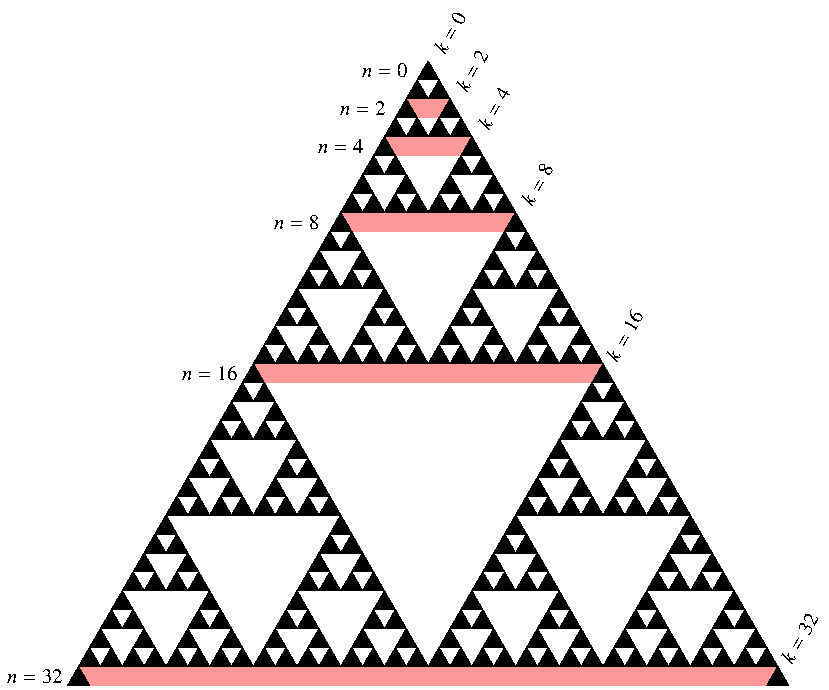
\includegraphics[width=\textwidth]{../../buch/chapters/30-endlichekoerper/images/binomial2.pdf}
\end{center}
\end{block}}
\end{column}
\end{columns}
\end{frame}
